\scanpage{31}
alors $\exists!\ j'\in I$ tel que
\[
\left\{\begin{aligned}
&j'\ne j\\
&j'\ \text{succ. de }i,\ k\ \text{succ. de }j'
\end{aligned}\right.
\]

\margin{$\downarrow\ \Rightarrow$}
d) \deleted{\unsure{$\forall$|tout}} $i\in I$, \inserted{$i$ non \unsure{minimum|minimal|minimiseur}} \deleted{\unsure{et non plus petit} \unsure{él.} $0$}
\[
\begin{aligned}
&i=\mathrm{Sup}\,(j\in I\mid j<i)\\
&i\ \text{non max-imal.}\Rightarrow \deleted{\unsure{\text{si }i\ne}}\ i=\mathrm{Inf}\,(j\in I\mid j>i)
\end{aligned}
\]

\uline{dim $-1$} \quad $I$ a un seul élément $(0=1)$.

\uline{dim $0$} \quad $I$ a deux éléments distincts ($0$ et $1$, \deleted{\unsure{$\exists$}} $0\ne1$)

\uline{dim $1$} \quad $I$ a \deleted{trois} quatre éléments $0$, $1$ et deux \unsure{int.|incomp.} $x,y$

( \deleted{$x,y$ \unsure{son}}

\diagram{\begin{tikzcd}[ampersand replacement=\&,column sep=small,row sep=small]
 \& 1 \arrow[dl,dash]\arrow[dr,dash] \&\\
 x \& \& y\\
 \& 0 \arrow[ul]\arrow[ur,dash] \&
\end{tikzcd}}

\uline{dim $2$}

\diagram{\(\begin{array}{lll}
\dim -1&0&\\
\dim 0&x_0\quad x_1\ldots x_{n-1}&\\
\dim 1&&\\
\dim 2&1&\begin{array}{l}\text{contours}\\\text{dont les comp.}\\\text{conn. ont au moins 3 sommets}\end{array}
\end{array}\)}

\figure{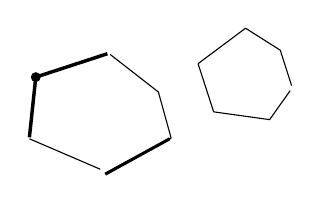
\begin{tikzpicture}[x=.9cm,y=.9cm,line join=round]
\draw[line width=1.25pt] (0,0)--(.09,.85)--(1.1,1.18);
\draw (1.14,1.17)--(1.82,.64)--(2,-.01)--(1.08,-.5);
\draw[line width=1.1pt] (1.07,-.52)--(1.98,-.02);
\draw (0,-.02)--(1,-.45);
\fill (.09,.85) circle (.07);
\draw (2.38,1.04)--(3.05,1.54)--(3.54,1.23)--(3.7,.73);
\draw (3.68,.66)--(3.39,.25)--(2.60,.36)--(2.38,1.04);
\end{tikzpicture}}

\uline{dim $3$} \quad On voudrait que si $x$ est un sommet

\diagram{\(\begin{array}{l|l}
-1&0\\0&\text{sommets}\\1&\text{arêtes}\\2&\text{faces}\\3&1
\end{array}\)}

% Double vertical rule between the table and the following text.
les $y>x$ \deleted{\unsure{qui le} \unsure{contiennent}}, \inserted{$y\ne1$,} forment un
contour \uline{connexe}

et si $x$ est une face
les $y<x$ \unsure{qq|que}, $y\ne0$,
forment un \uline{contour}
$(\pi_0\unsure{\simeq|=}0)$

\uline{dim $4$}
% archive sheet number: 30
